\chapter{Diseño del sistema}
En esta sección se va a mostrar el diseño de la aplicación. Se detallará sobre el modelo de datos, aspectos de seguridad y diseño visual de la aplicación.

\subsection{Modelo de datos}
Para poder empezar con la implementación es de vital importancia definir cuáles son los datos que vamos a manipular en la aplicación, que entidades representan y como se relacionan estas entidades.

    \begin{figure}[H]
        \centering
        \includegraphics[width=0.9\linewidth]{images/diagramaLógicoV3.png}
        \caption{Modelo lógico de datos}
        \label{fig:diagramaER}
    \end{figure}

% Para facilitar la explicación de lo anterior mencionado nos referiremos a la figura \ref{fig:diagramaER}
\subsubsection{Usuario}
Un usuario representa a una persona que utiliza la aplicación. Cada usuario tiene un identificador único, un nombre, una dirección de correo electrónico, una contraseña, un nombre de usuario, una marca de tiempo de cuando se unió a la aplicación, y una ubicación preferida.

\subsubsection{Grupo}
Un grupo es una entidad que representa un conjunto de usuarios que se han unido para comunicarse y colaborar. Cada grupo tiene un identificador único, un nombre, una descripción, un límite de miembros, lugar y tipo de grupo. También el grupo mantiene la referencia al usuario dueño del grupo.

\subsubsection{Mensaje}
Un mensaje es una entidad que representa la comunicación entre usuarios dentro de un grupo.Cada mensaje mantiene una referencia al grupo y al usuario que lo envió, el contenido del mensaje, una marca de tiempo de cuando se envió. Cada mensaje también mantiene una lista con las referencias de los usuarios que han leído dicho mensaje.

\subsubsection{Membresía}
La membresía es una entidad intermedia que representa la relación entre los usuarios y los grupos. Es decir, denota que un usuario se ha unido a un grupo. Cada membresía tiene un identificador único, el identificador del usuario, el identificador del grupo, y una marca de tiempo de cuando el usuario se unió al grupo.

\subsubsection{Evento}
El entidad evento viene siempre asociada a un grupo, este describe el encuentro de grupo. Mantiene campos como título, descripción, marca de tiempo, fecha de celebración y un campo booleano que identifica la flexibilidad horaria.

\subsubsection{Asistencia}
La asistencia como su nombre indica, identifica la asistencia de un usuario a un evento. Tiene un identificador compuesto por dos claves foráneas, en este caso los identificadores de evento y usuario. Así como dos campos opcionales de tipo marca de tiempo que identifican la preferencia del tiempo de comienzo y final del evento en el caso en el que este último permita la flexibilidad horaria.

\begin{comment}
\subsection{Aspectos de Seguridad}
Es importante considerar aspectos de seguridad en el diseño de la aplicación. Por ejemplo, las contraseñas de los usuarios deben ser almacenadas de manera segura utilizando métodos de hash y sal. Además, debería haber autenticación y autorización adecuadas para asegurar que los usuarios solo puedan realizar acciones que les estén permitidas, como por ejemplo, un usuario solo puede eliminar un grupo si es el dueño de este.
\end{comment}

\subsection{Navegación}
\begin{figure}[H]
        \centering
        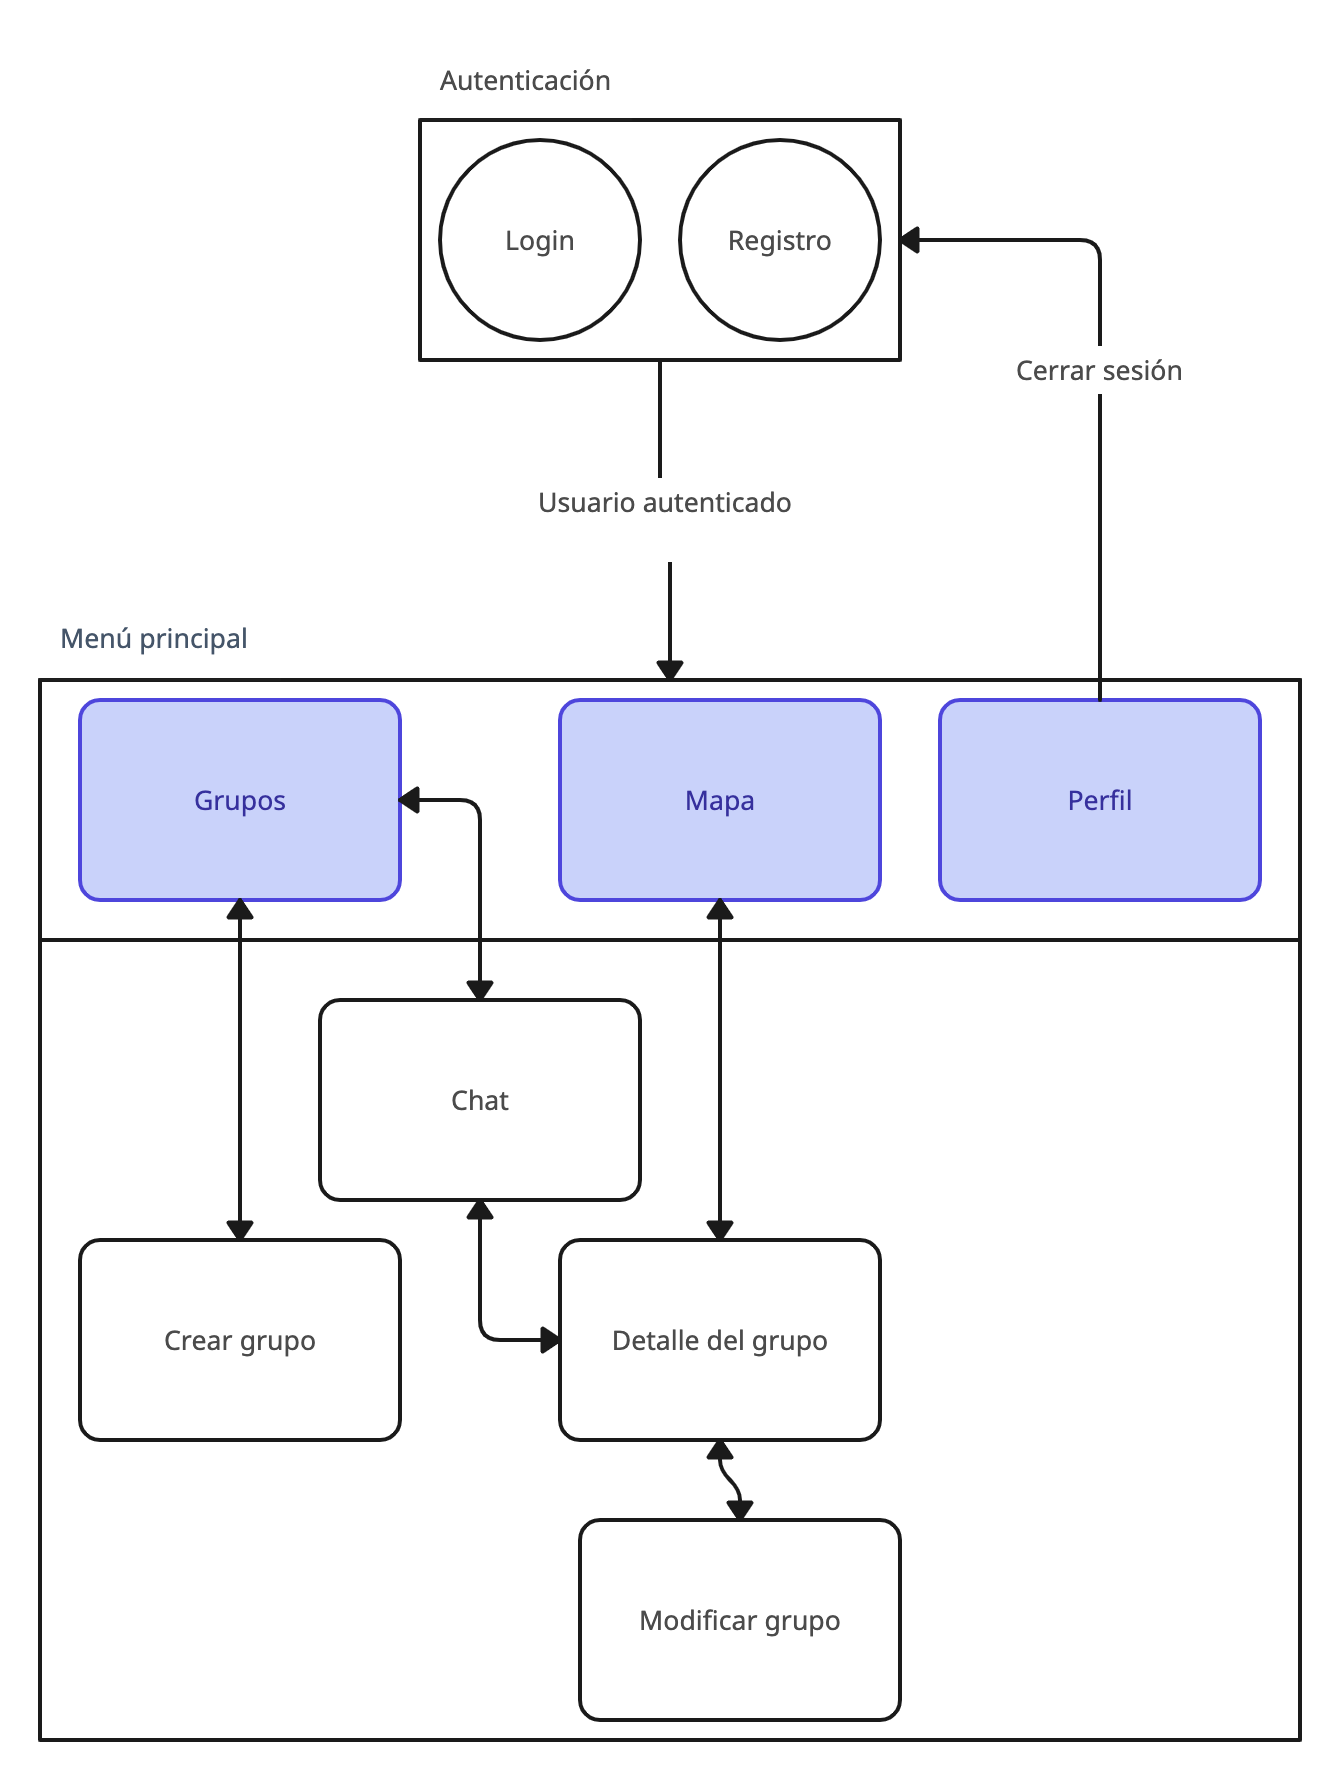
\includegraphics[width=1\linewidth]{images/navegacion.png}
        \caption{Diagrama de navegación}
        \label{fig:diagramaER}
\end{figure}
La vistas de la aplicación se han encapsulado en distintos grupos:

\subsubsection{Login}
La pantalla \textit{Login} es el primer punto de entrada de nuestra aplicación, dónde el usuario puede tomar varias acciones: autenticarse, proceder al registro o restablecer contraseña.

\begin{figure}[H]
        \centering
        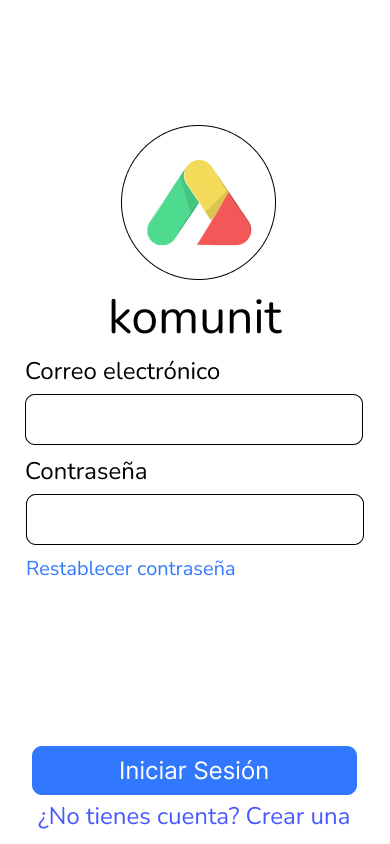
\includegraphics[cframe=black 2pt,width=0.3\linewidth]{images/vistas/Login.png}
        \caption{Diagrama de navegación}
        \label{fig:Vista Login}
\end{figure}

\subsubsection{Registro}
La vista de registro en donde el visitante procederá a rellenar sus datos tales como nombre, correo ele
\begin{figure}[H]
        \centering
        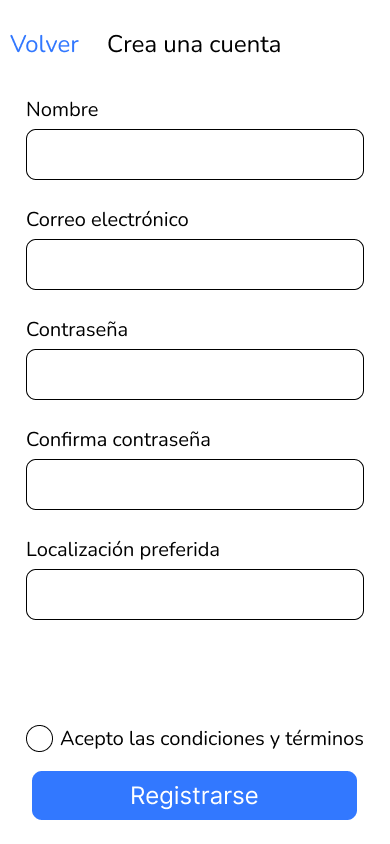
\includegraphics[cframe=black 2pt,width=0.3\linewidth]{images/vistas/CrearCuenta.png}
        \caption{Diagrama de navegación}
        \label{fig:Vista Resgistro}
\end{figure}
\subsubsection{Confirmación de correo electrónico}
\begin{figure}[H]
        \centering
        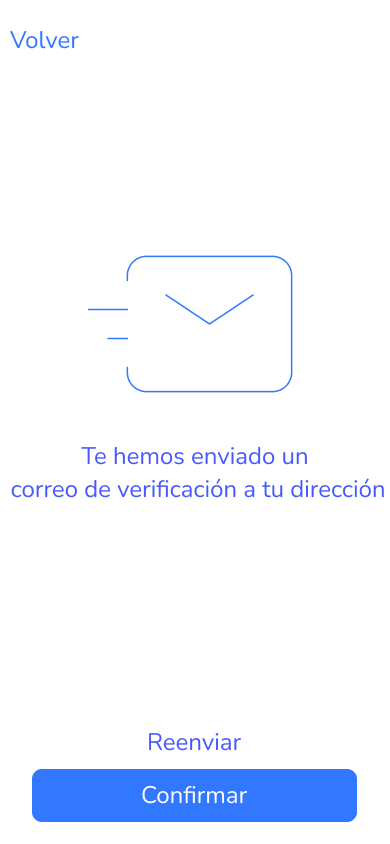
\includegraphics[cframe=black 2pt,width=0.3\linewidth]{images/vistas/Confirmación de correo.png}
        \caption{Diagrama de navegación}
        \label{fig:Vista Confirmación Correo Electrónico}
\end{figure}
\subsubsection{Mapa}
\begin{figure}[H]
        \centering
        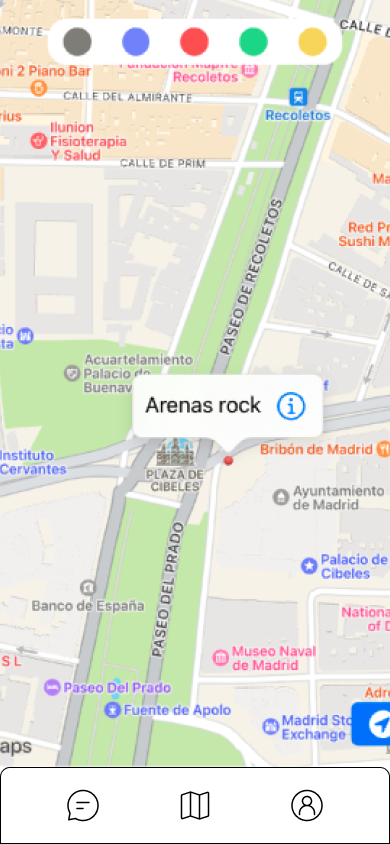
\includegraphics[cframe=black 2pt,width=0.3\linewidth]{images/vistas/VistaMapa.png}
        \caption{Diagrama de navegación}
        \label{fig:Vista mapa}
\end{figure}
\subsubsection{Lista de grupos}
\begin{figure}[H]
        \centering
        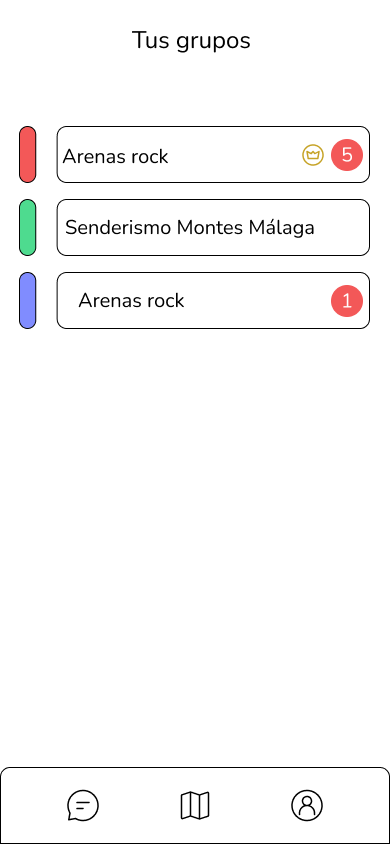
\includegraphics[cframe=black 2pt,width=0.3\linewidth]{images/vistas/Lista grupos.png}
        \caption{Diagrama de navegación}
        \label{fig:Vista grupos}
\end{figure}
\subsubsection{Chat}
\begin{figure}[H]
        \centering
        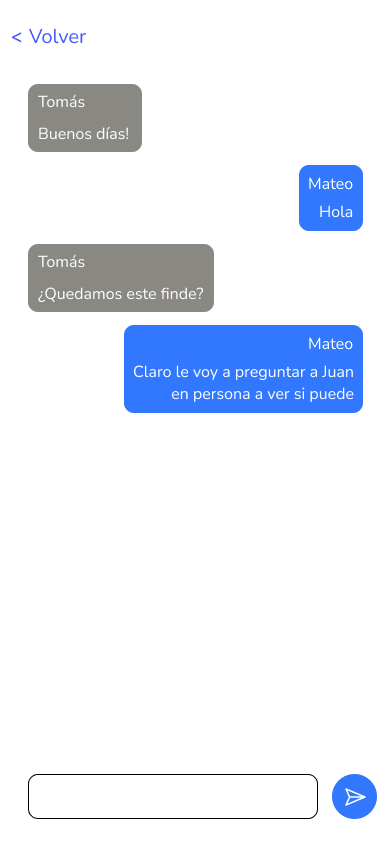
\includegraphics[cframe=black 2pt,width=0.3\linewidth]{images/vistas/ChatGrupo.png}
        \caption{Diagrama de navegación}
        \label{fig:Vista chat grupo}
\end{figure}
\subsubsection{Detalle del grupo}
\begin{figure}[H]
        \centering
        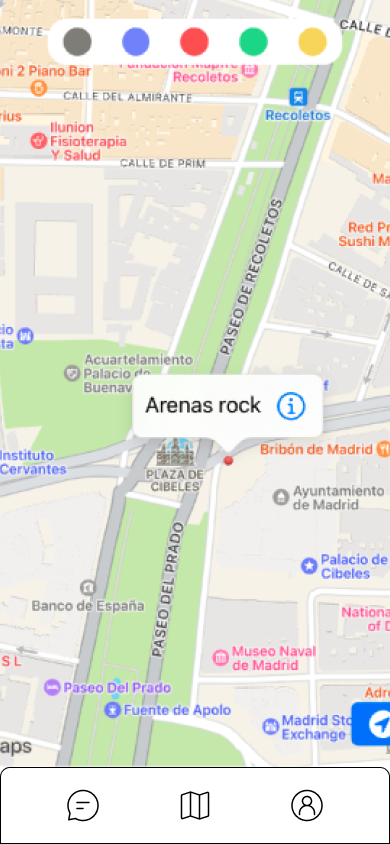
\includegraphics[cframe=black 2pt,width=0.3\linewidth]{images/vistas/VistaMapa.png}
        \caption{Diagrama de navegación}
        \label{fig:Vista detalle del grupo}
\end{figure}
\subsubsection{Crear grupo}
\begin{figure}[H]
        \centering
        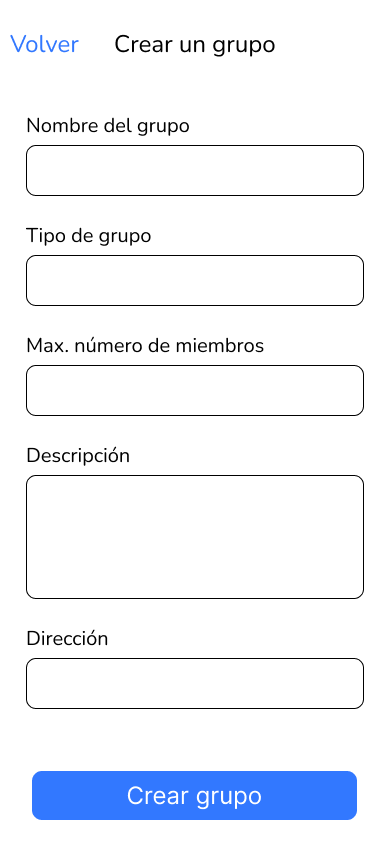
\includegraphics[cframe=black 2pt,width=0.3\linewidth]{images/vistas/CrearGrupo.png}
        \caption{Diagrama de navegación}
        \label{fig:Vista Crear Grupo}
\end{figure}
\subsubsection{Perfil}
\begin{figure}[H]
        \centering
        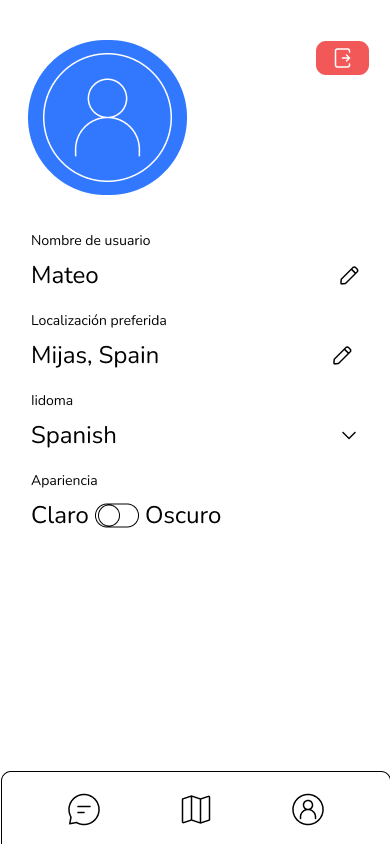
\includegraphics[cframe=black 2pt,width=0.3\linewidth]{images/vistas/PerfilUsuario.png}
        \caption{Diagrama de navegación}
        \label{fig:Vista Perfil}
\end{figure}





